\documentclass[10pt,portuguese]{article}

\usepackage{fourier}

\usepackage[]{graphicx}
\usepackage[]{color}
\usepackage{xcolor}
\usepackage{alltt}
\usepackage{listings}
\usepackage[T1]{fontenc}
\usepackage[utf8]{inputenc}
\setlength{\parskip}{\smallskipamount}
\setlength{\parindent}{5ex}
\usepackage{indentfirst}
\usepackage{listings}
\usepackage{setspace}
\usepackage{hyperref}
\hypersetup{
    colorlinks=true,
    linkcolor=auburn,
    filecolor=magenta,      
    urlcolor=blue, urlsize=2em
}

% Set page margins
\usepackage[top=100pt,bottom=100pt,left=68pt,right=66pt]{geometry}

% Package used for placeholder text
\usepackage{lipsum}

% Prevents LaTeX from filling out a page to the bottom
\raggedbottom


\usepackage{fancyhdr}
\fancyhf{} 
\fancyfoot[C]{\thepage}
\renewcommand{\headrulewidth}{0pt} 
\pagestyle{fancy}

\usepackage{titlesec}
\titleformat{\chapter}
   {\normalfont\LARGE\bfseries}{\thechapter.}{1em}{}
\titlespacing{\chapter}{0pt}{50pt}{2\baselineskip}

\usepackage{float}
\floatstyle{plaintop}
\restylefloat{table}

\usepackage[tableposition=top]{caption}



\frontmatter

\definecolor{light-gray}{gray}{0.95}

\renewcommand{\contentsname}{Índice}

\begin{document}

\selectlanguage{portuguese}

\begin{titlepage}
	\clearpage\thispagestyle{empty}
	\centering
	\vspace{2cm}

	
	{\Large  Sistemas Operativos \par}
	\vspace{0.5cm}
	{\small Professor: \\
	José Nuno Panelas Nunes Lau\par}
	\vspace{4cm}
	{\Huge \textbf{Estatísticas de Utilizadores em Bash}} \\
	\vspace{1cm}
	\vspace{4cm}
	{\normalsize Carolina Araújo, 93248 \\ 
	             Hugo Paiva, 93195
	   \par}
	   	{\tiny
	Igual distribuição de trabalho \\entre os dois membros\par}
	\vspace{2cm}

    
\includegraphics[scale=0.20]{images/logo_ua.png}
    
    \vspace{2cm}
    
	{\normalsize DETI \\ 
		Universidade de Aveiro \par}
		
	{\normalsize 29-11-2019 \par}
	\vspace{2cm}
		
	
	\pagebreak

\end{titlepage}
\tableofcontents{}
\clearpage

\section{Introdução}
\par Este trabalho prático foi baseado no desenvolvimento de scripts em Bash que permitem recolher algumas estatísticas sobre o modo como os utilizadores estão a usar o sistema computacional. 

\par Estas ferramentas permitem visualizar o número de sessões e o tempo total de ligação para uma selecção de utilizadores e um determinado período de tempo, permitindo também a comparação dos dados obtidos em períodos distintos.

\par Para desenvolver estas ferramentas com os resultados expectáveis é necessário compreender o funcionamento da Bash. Sendo mantida pelo famoso projeto GNU, a Bash, é uma ferramenta extremamente eficiente encontrada na maioria dos sistemas baseados em UNIX. É também altamente personalizável e, por isso, muito usada no mundo da programação.
 

\clearpage

\section{Preparação}
\par Antes de avançar com qualquer desenvolvimento em código, procedeu-se à cópia do ficheiro "/var/log/wtmp" do computador da sala de aula. Este ficheiro contém o histórico atual de todos os logins e logouts associados ao computador em questão, fornecendo todos os dados necessários para o desenvolvimento dos scripts. Desta forma, foi permitida a sua leitura, durante a implementação, sem necessidade de se estar conectado ao computador nas instalações do DETI.
\par Um dos membros do grupo, devido a possuir um Macbook, apenas dispunha da versão 3 da Bash. Sendo esta versão de 2007, várias funcionalidades que viriam a ser utilizadas durante o trabalho não eram suportadas. Um exemplo disto são os \textit{Arrays Associativos} que apenas são suportados a partir da versão 4 da Bash, versão esta que está instalada nos computadores do DETI. Este problema foi resolvido através da utilização de uma máquina virtual de ambiente Linux.


\clearpage

\section{Estatísticas dos utilizadores}
O script criado (\textit{userstats.sh}) permite a visualização filtrada das estatísticas dos utilizadores contidas no ficheiro "/var/log/wtmp". Após a sua execução, é possível observar o número de sessões, tempo total de ligação (em minutos), duração máxima e duração mínima das sessões dos utilizadores selecionados, no período desejado.

\subsection{Estrutura}
\par Inicialmente, o grupo começou o trabalho utilizando apenas \textit{Arrays} para armazenar e tratar os dados. Após a descoberta dos \textit{Arrays Associativos} e a facilidade que este dispõem em associar, neste caso, os utilizadores com a informação dos mesmos, foi estabelecida a estrutura final onde os dados iriam ser tratados.
\par Posto isto, foram criados dois \textit{Arrays Associativos} e um \textit{Array} para simplificar o tratamento dos dados.

\begin{figure}[!h]
    \centering
    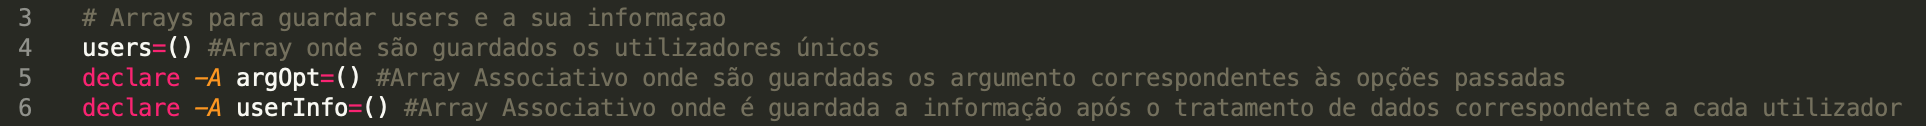
\includegraphics[width=\textwidth]{estrutura.png}
    \caption{\textbf{\textit{Arrays}} mais relevantes na implementação deste script}
\end{figure}
\newline
 \begin{itemize}
   \item {\textbf{users}}   - \textit{Array} onde são guardados os utilizadores, sem repetição, durante o tratamento de dados;
   \\
   \item {\textbf{argOpt}}  - \textit{Array Associativo} onde são guardadas as opções e os respetivos argumentos durante o tratamentos de opções;
   \\
   \item {\textbf{userInfo}}- \textit{Array Associativo} onde são guardadas as informações tratadas durante o tratamento de dados.
 \end{itemize}
\newline
 \par Ao armazenar a informação desta forma, principalmente devido aos \textit{Arrays Associativos}, o tratamento de dados, tal como a impressão dos mesmo são muito mais facilitada.

\clearpage

\subsection{Tratamento de Opções}

\par As opções foram tratadas usando o comando shell \textit{getopts}, abordado nas aulas práticas. Este comando analisa os argumentos passados na Bash e, se estes estiverem definidos na sua criação, são efetuadas as tarefas desejadas.
\newline
\par O tratamento de opções é iniciado com a chamada da função \textbf{\textit{args()}}.
\begin{figure}[!h]
    \centering
    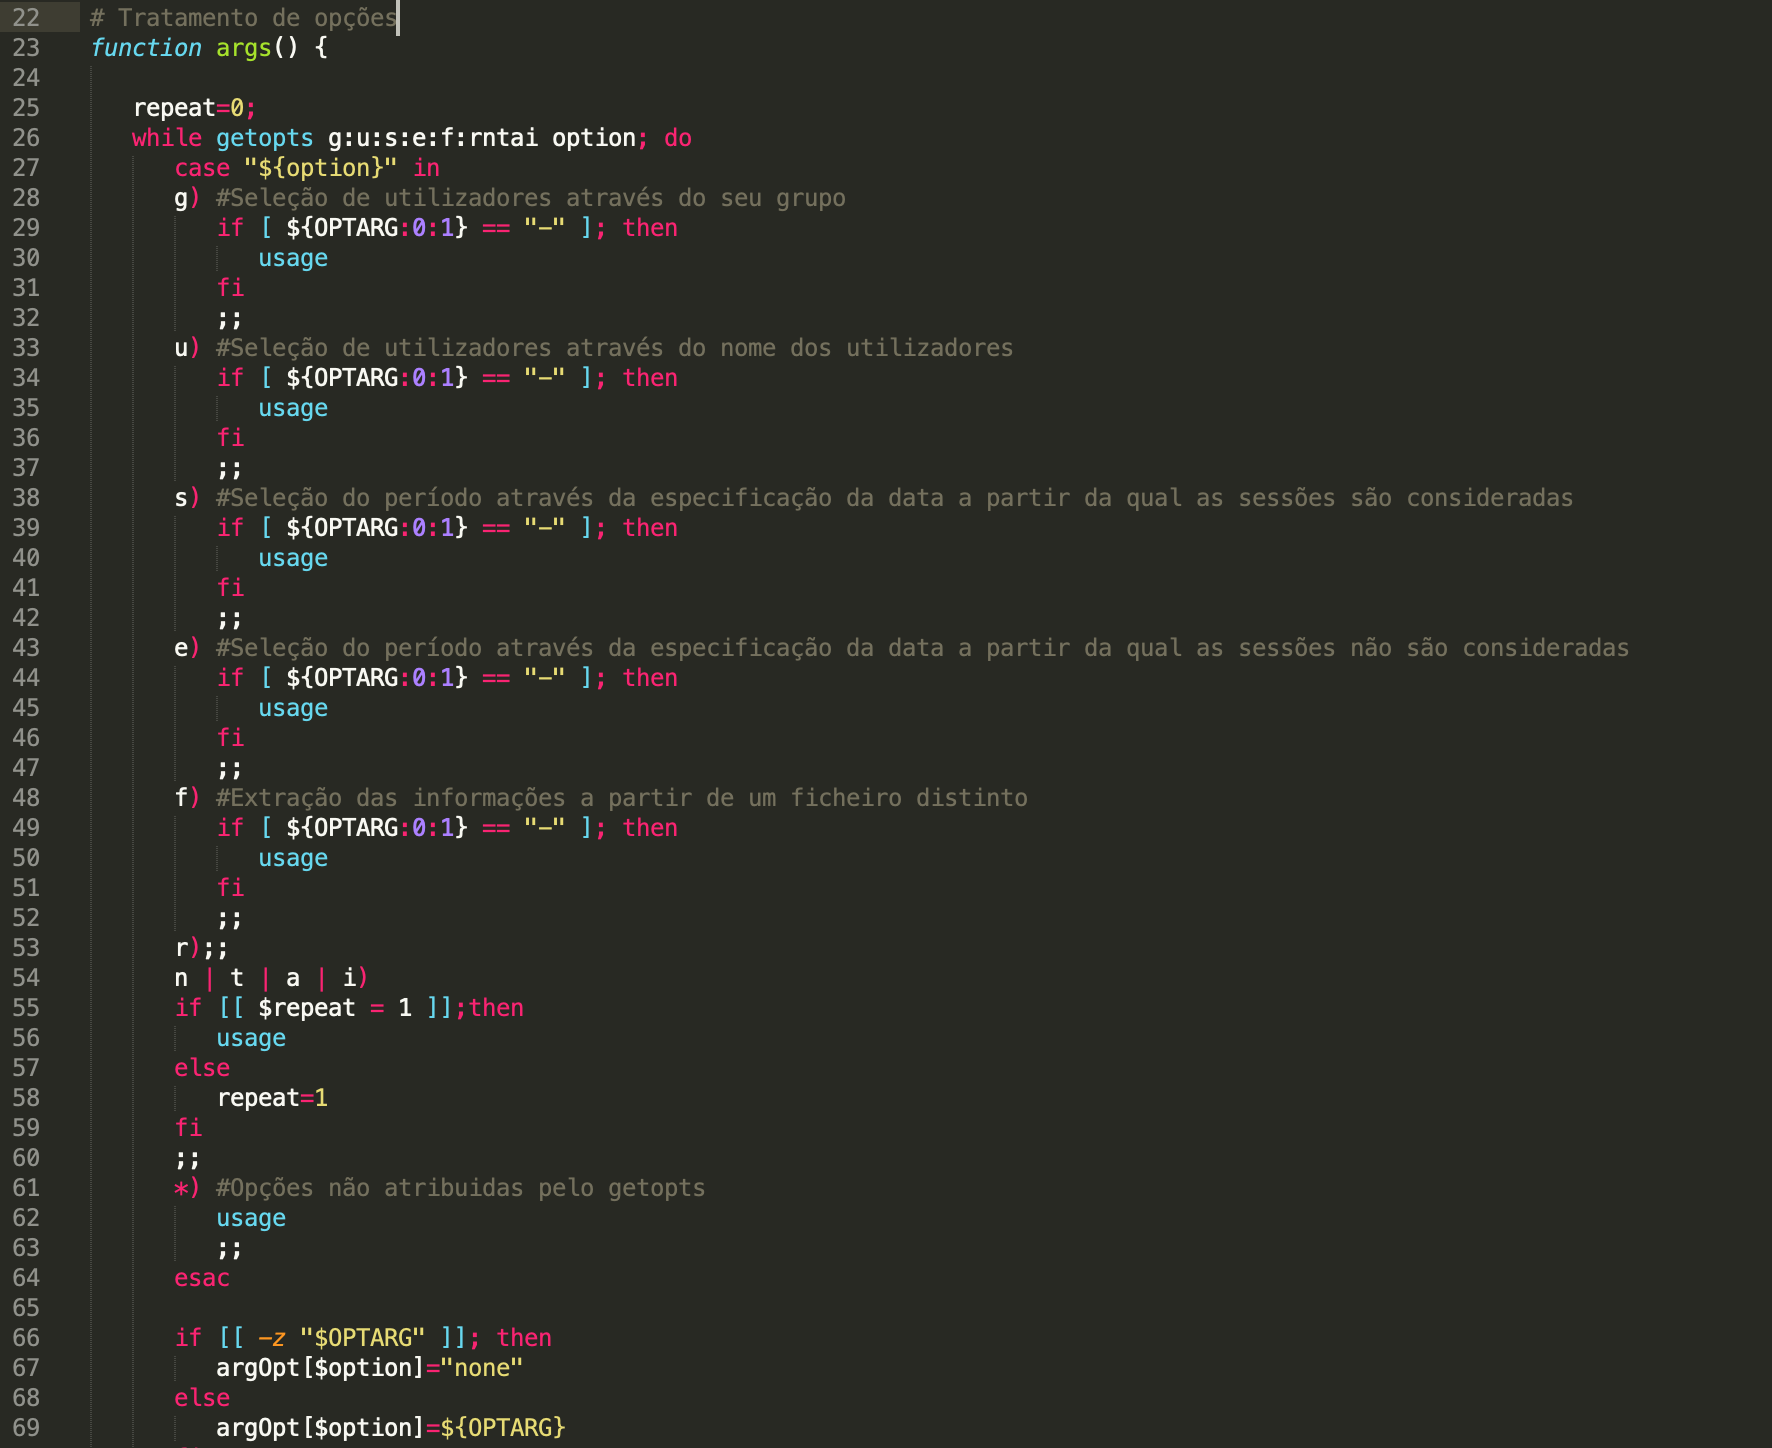
\includegraphics[width=\textwidth]{getopts.png}
    \caption{Função \textbf{\textit{args()}} que procede ao tratamento de opções}
\end{figure}
\par O \textit{getopts} recebe parâmetros (\textit{g:u:s:e:f:rntai}) que correspondem às opções que o comando aceita. As opções \textit{-g}, \textit{-u}, \textit{-s}, \textit{-e} e \textit{-f} recebem argumentos pois estão seguidas de dois pontos ':'. Estando este comando dentro de um \textit{while}, é repetido as vezes necessárias para percorrer todas as opções e argumentos introduzidos no terminal, aquando a chamada do programa. As opções são guardadas, em cada ciclo, na variável \textit{option} sendo executado o código associado a cada opção, consoante o \textit{case statement}.
\par Nas opções válidas que recebem argumentos foi feita uma verificação se o argumento introduzido não é uma outra opção (por erro do utilizador). Isto é feito comparando o 1º caractere do argumento com \textit{'-'}, executando a função \textit{usage} quando esta comparação é verificada, significando que é uma outra opção.
\par Para as opções \textit{-n}, \textit{-t}, \textit{-a} e \textit{-i} que não podem ser repetidas, foi criada uma variável \textit{repeat} para averiguar se alguma destas variáveis já foi passada à função. Em caso afirmativo, é executada a função \textbf{\textit{usage()}}.
\par Sempre que é introduzida uma opção inválida ou de forma incorreta, o \textit{case statement} executa a função \textbf{\textit{usage()}}, que indica a forma de utilização do script.
\begin{figure}[!h]
    \centering
    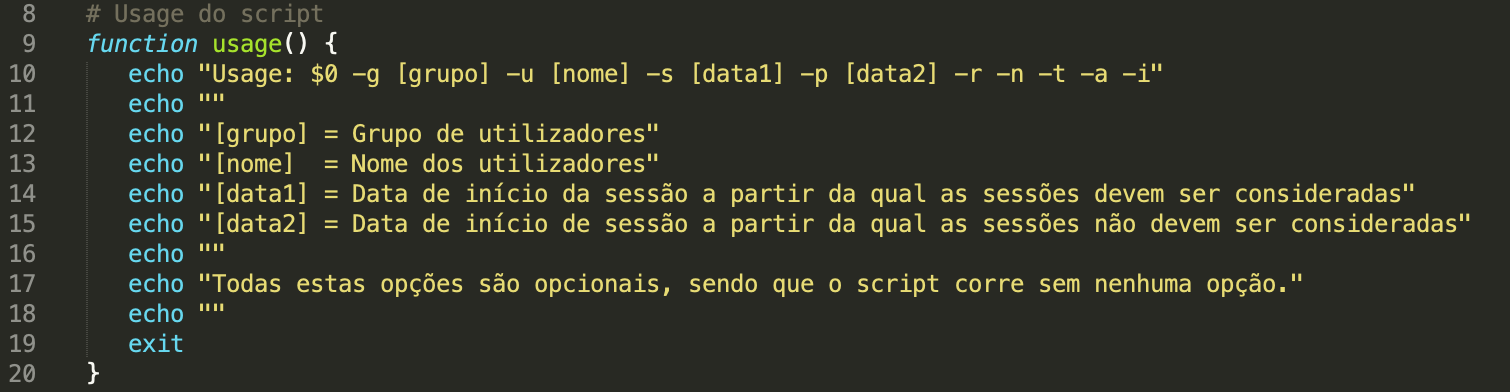
\includegraphics[width=\textwidth]{usage.png}
    \caption{Função \textbf{\textit{usage()}} que refere as opções e argumentos esperados}
\end{figure}
\newline
\par Ainda dentro do ciclo \textit{while}, são executadas averiguações para guardar as opções e os respetivos argumentos numa das estruturas de dados definidas anteriormente. Se for passada uma opção válida mas nenhum argumento, ou seja, a variável \textit{OPTARG} está vazia, a opção \textit{-z} da expressão condicional retorna \textit{true} e é guardado no \textit{Array Associativo} \textit{argOpt} a opção em questão (\textit{key}) e o valor \textit{"none"} (\textit{value}). Ao passar uma opção válida com um argumento, é guardada na mesma estrutura de dados a opção em questão (\textit{key}) e o valor do argumento (\textit{value}).
\begin{figure}[!h]
    \centering
    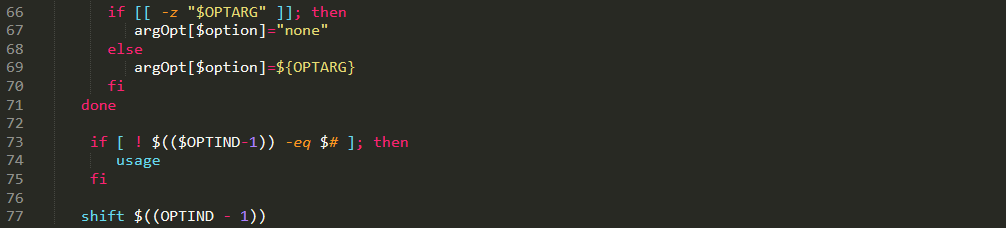
\includegraphics[width=\textwidth]{optarg.png}
    \caption{Verificação da inexistência de argumento associado à atual opção}
\end{figure}
\newline
\par Já fora do ciclo while, é executada a verificação se \textit{\$((OPTIND-1))} é igual ao número de argumentos passado à função. Visto que a variável \textit{OPTIND} corresponde às opções e argumentos aceites no \textit{getopts}, incluindo o nome do ficheiro, e \textit{\$\#} corresponde ao número de argumentos passados ao script, com exceção do nome do ficheiro, é \textbf{subtraído um} ao \textit{OPTIND} de modo a comparar o que foi aceite no \textit{getopts} e o que não, executando a função \textit{usage} no caso de argumentos a mais.
\par Por fim, \textit{\$((OPTIND-1))} vai remover todas as opções que foram passadas pelo \textit{getopts}, nos seus parâmetros. Desta forma, \textit{\$1} vai referir o primeiro argumento passado ao script, que não é uma opção.


\clearpage 

\subsection{Leitura e tratamento de dados}
\newline
\par O tratamento de dados é iniciado com a chamada da função \textbf{\textit{getUsers()}}.
\begin{figure}[!h]
    \centering
    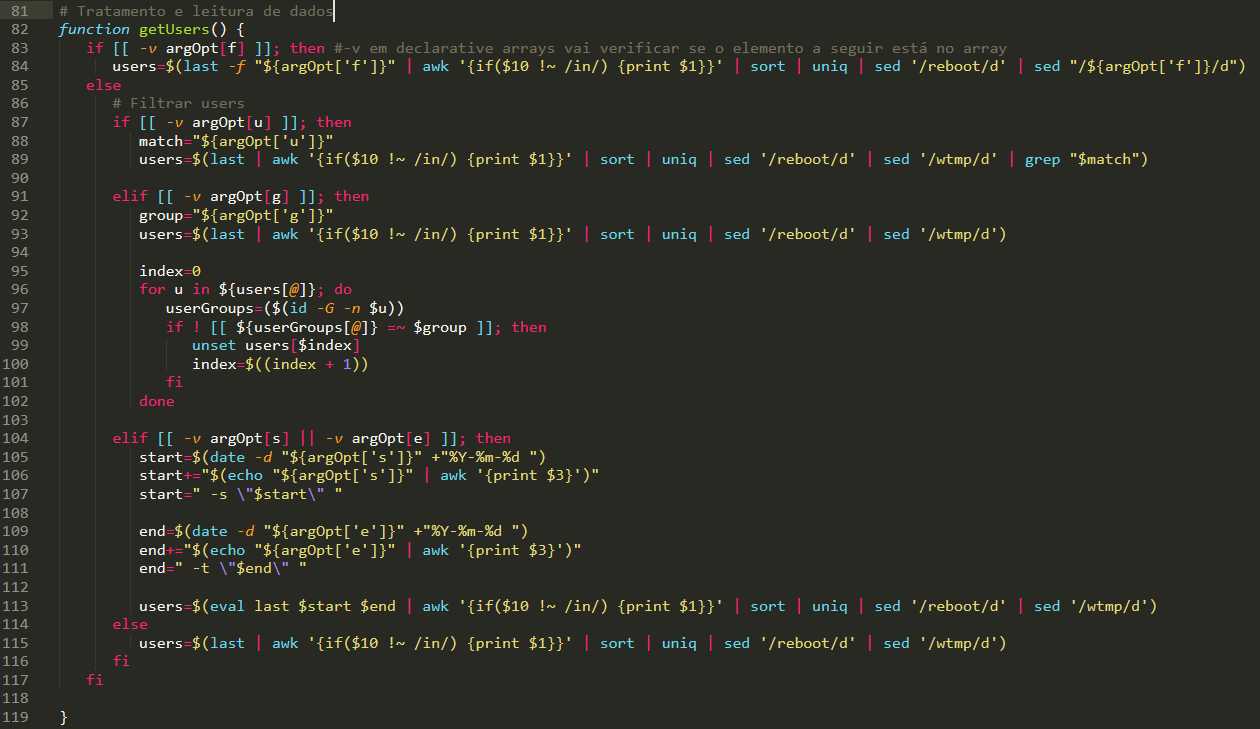
\includegraphics[width=\textwidth]{getUsers.PNG}
    \caption{Função \textbf{\textit{getUsers()}} que seleciona os utilizadores que são guardados no \textit{Array} \textit{users}}
\end{figure}
\par De modo a aumentar a eficiência e, desta forma, diminuir o tempo de execução do programa, foi decidido filtrar os utilizadores pretendidos nesta função, guardando-os num \textit{Array}. Assim, qualquer próxima função precisa apenas de iterar sobre os utilizadores, já previamente selecionados, para obter informação relativa aos mesmos.
\par Consoante os argumentos passados no terminal e através de comandos Linux como \textit{grep}, \textit{awk}, \textit{sed}, \textit{sort} e \textit{uniq} foi-nos possível filtrar somente utilizadores únicos que correspondessem a uma determinada expressão \textit{RegEx}, assim como apenas aqueles de um ficheiro específico, os de um certo grupo ou utilizadores que tivessem iniciado sessão entre certas datas.
\par A lógica geral de funcionamento desta função passa por chamar apenas uma vez o comando \textit{last}, com base nas opções passadas no terminal, de modo a obter o seu \textit{output} e então selecionar apenas a informação que nos é conveniente.
\par Através do comando \textit{awk} é possível obter somente os elementos na posição \textit{\$1} caso estes não correspondam a um utilizador ainda conectado ao computador em questão. Essa verificação faz-se com um \textit{if} que testa se os elementos na posição \textit{\$10} correspondem à palavra "in".
\par Os comandos \textit{sort} e \textit{uniq} garantem a salvaguarda apenas dos utilizadores únicos. São, ainda, capazes de retirar aqueles cujo elemento na posição \textit{\$1} corresponda a "reboot" ou ao nome do ficheiro (passado no terminal ou então, por default, o ficheiro "/var/log/wtmp"), com a chamada do comando \textit{sed}. 
\par Se é passada a opção "-f" no terminal, o comando \textit{last} é chamado juntamente com "-f <filename>". Enquanto que, se forem passadas as opções "-s" e "-e",  procede-se à transformação das strings passadas como datas, de modo a ficarem no formato \textbf{YYYY}-\textbf{MM}-\textbf{DD} \textbf{hh}:\textbf{mm} e, posteriormente, o \textit{last} será chamado com as opções "-s" e "-t" (\textit{last} -s <date1> -t <date2>), utilizando \textit{eval}, uma vez que este comando serve para construir um outro comando, concatenando argumentos.
\par No caso da opção "-u" ter sido passada no terminal, utiliza-se o comando \textit{grep "\$match"}, de forma a que somente utilizadores cuja string identificadora do seu nome corresponda à expressão passada no terminal, fiquem armazenados no \textit{Array} \texit{users}. Essa tal expressão terá sido guardada no elemento \textit{\$match} (correspondente ao valor associado à opção "-u")
\par \textbf{Nota:} As aspas em torno da variável \textit{\$match} na opção "-u" foram colocadas uma vez que, aquando da realização de testes finais, notou-se que a chamada do programa com as opções "  \textbf{-n -u ".*"  }" dava um output diferente do esperado, sendo que, com qualquer outra expressão \texit{RegEx}, o programa imprimia o esperado. Após alguma pesquisa chegamos à conclusão de que seria necessário colocar estas aspas.
\par Por fim, caso seja indicada a opção \textit{"-g"}, atribui-se à variável \textit{group} o valor passado como argumento desta opção, isto é, o grupo que se deseja filtrar. Da mesma maneira que, como nas outras opções, vai-se buscar todos os utilizadores únicos, iterando-os, para ver quais deles pertencem ao grupo especificado. Ver a que grupos pertence cada utilizador faz-se através do comando \textit{id -G -n <utilizador>}, cuja opção \textit{"-G"} torna mandatório imprimir apenas os grupos suplementares e \textit{"-n"}, como opção prévia, imprime o nome dos grupos e utilizadores em vez dos seus IDs. Posto isto, caso nenhum dos grupos do utilizador em questão seja igual ao grupo agora guardado na variável \textit{group}, recorrendo ao comando \textit{unset}, esse usuário será retirado do \textit{Array} \textit{users}. A variável \textit{index} serve para aceder aos elementos indesejados, sendo que, após a retirada de um dos mesmos, esta variável é sempre incrementada. 
\newpage
\par Seguidamente a informação obtida passa para a função \textbf{\textit{getUserInfo()}}.
\begin{figure}[!h]
    \centering
    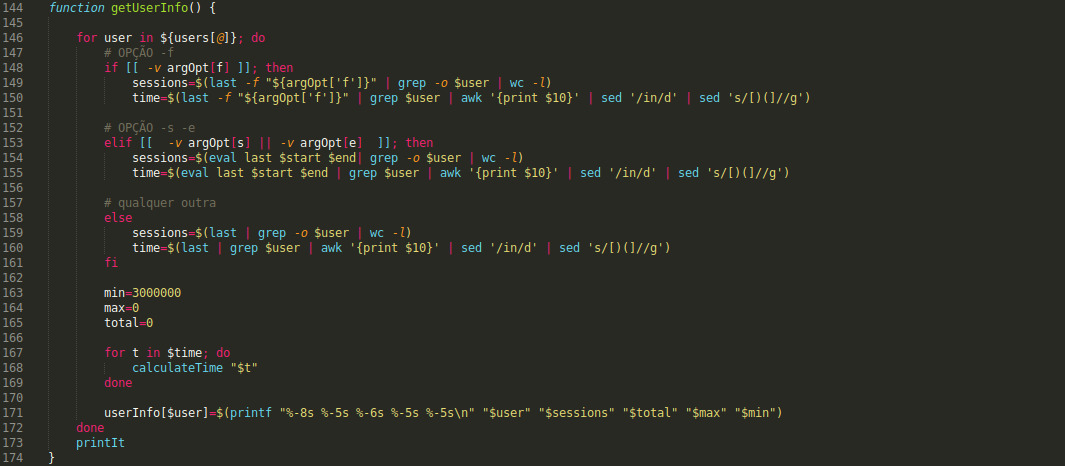
\includegraphics[width=\textwidth]{getUsersInfo.jpeg}
    \caption{Função \textbf{\textit{getUserInfo()}} que utiliza o \textit{Array} \textit{users} para obter a informação relativa a cada utilizador}
\end{figure}
\par Para cada utilizador filtrado na função anterior, esta vai contar o número de sessões e o tempo total, mínimo e máximo de ligação para cada sessão de cada utilizador. Isto é feito com auxílio aos comandos \textit{last  |  grep}, que selecionam a informação do \textit{last}, de modo a que o utilizador seja iterado pelo ciclo \textit{for}, passando-o como argumento do \textit{grep}, sendo ainda possível ir buscar informação a um ficheiro, caso seja passada a opção \textit{"-f"} no terminal.
\par O comando \textit{wc -l} conta o número de linhas onde aparece esse utilizador, revelando assim o número de sessões para cada um.
\par No caso do tempo de ligação de uma dada sessão, utiliza-se também o \textit{grep} e o \textit{awk} para ir buscar a informação na posição \textit{\$10} (o tempo decorrido em sessão), utilizando o \textit{sed} para remover os parênteses em torno do valor que realmente queremos, passando esta informação final para o \textit{Array} \textit{time}.
\par Caso tenham sido selecionadas as opções \textit{"-s"} e \textit{"-e"}, vamos buscar a informação formatada anteriormente para a data-ínicio e a data-final, chamando novamente o comando \textit{last} com recurso ao \textit{eval}, obtendo assim apenas as sessões e tempos de ligação entre as datas em questão.
\par São definidos valores iniciais de tempo máximo, mínimo e total de ligação do utilizador em questão e cada valor do \textit{Array} de tempos de cada ligação é passado à função \textbf{\textit{calculateTime()}}. Esta acaba por retornar já estes valores calculados, usando os anteriormente definidos para realizar comparações e, por fim, toda esta informação é colocada dentro de um \textit{Array Associativo}, cuja \textit{key} é o utilizador e o \textit{value} é já a informação final formatada numa string, com espaçamento e alinhamento definidos.
\newpage
\par Função \textbf{\textit{calculateTime()}}, chamada na função \textbf{\textit{getUsersInfo()}} 
\begin{figure}[!h]
    \centering
    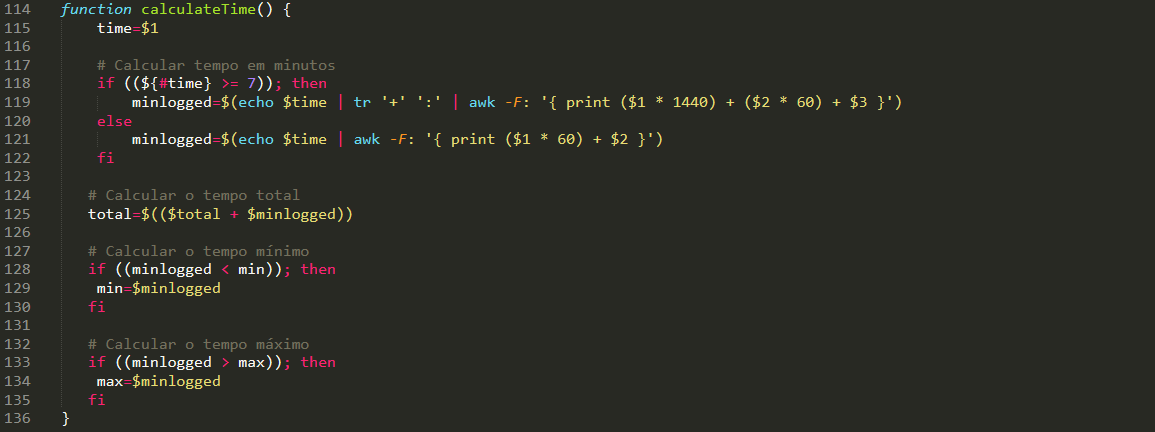
\includegraphics[width=\textwidth]{calculateTime.png}
    \caption{Função \textbf{\textit{calculateTime()}} que calcula o tempo máximo, mínimo e total para dado utilizador, com base no \textit{Array} \textit{time}}
\end{figure}
\par Para facilitar o entendimento do código, deu-se o nome de \textit{time} ao argumento passado à função, que é um dado elemento do \textit{Array} de tempos calculado para cada utilizador.
\par O argumento \textit{time} pode estar no formato \textbf{dd}+\textbf{hh}:\textbf{mm} ou apenas \textbf{hh}:\textbf{mm}. O primeiro contêm a informação de que o tempo daquela sessão foi \textbf{dd} dias, \textbf{hh} horas e \textbf{mm} minutos, enquanto que o segundo não chega a 24h de ligação, indicando apenas o número de horas e minutos gastos. Com base nisto, qualquer tempo cujo \textit{length} total seja superior a 7, significa que transporta a informação de um certo número de dias, portanto, substitui-se o '+' por ':' através do comando \textit{tr}, de modo a que o \textit{awk -F:} possa ir buscar a informação contida no elemento time e separa-la em cada ':' que encontrar. Assim, somos deixados com 3 argumentos (\textit{\$1}, \textit{\$2} e \textit{\$3}), indicando, cada um, respetivamente, o número de dias, horas e minutos dessa sessão. Com isto, basta multiplicar o número de dias, \textit{\$1}, por 1440 (o número de minutos/dia), multiplicar \textit{\$2} por 60 (o número de minutos/hora) e somar ambos esses resultados com o valor de minutos, \textit{\$3}), obtido pelo \textit{awk}. Caso o \textit{length} do elemento seja inferior a 7, significa que não indica número de dias, ou seja, não é necessário substituir nenhum sinal '+', visto que não há. De resto a informação é processada de modo bastante semelhante. O resultado obtido de qualquer um destes procedimentos é armazenado na variável \textit{minlogged}. 
\par De seguida, acrescenta-se à variável total de um dado \textit{user}, o número de minutos calculado (\textit{minlogged}). Compara-se também este valor aos tempos mínimos e máximos até então desse mesmo utilizador. Desta forma, verifica-se se o \textit{minlogged} é inferior ao valor da variável \textit{min} ou superior ao valor da variável \textit{max}, podendo ser atualizado o valor de uma das duas variáveis, caso um dos casos se verifique.
\par Assim sendo, garante-se que todos os valores de tempos de cada sessão de um dado utilizador são comparados, podendo devolver a informação de qual é o tempo total de ligação, o tempo mínimo e o tempo máximo, como pretendido.
\clearpage

\subsection{Impressão ordenada dos dados filtrados}
\par A impressão ordenada dos dados filtrados é feita com a chamada da função \textbf{\textit{printIt()}}, que é chamada na função \textbf{\textit{getUsers()}}.
\begin{figure}[!h]
    \centering
    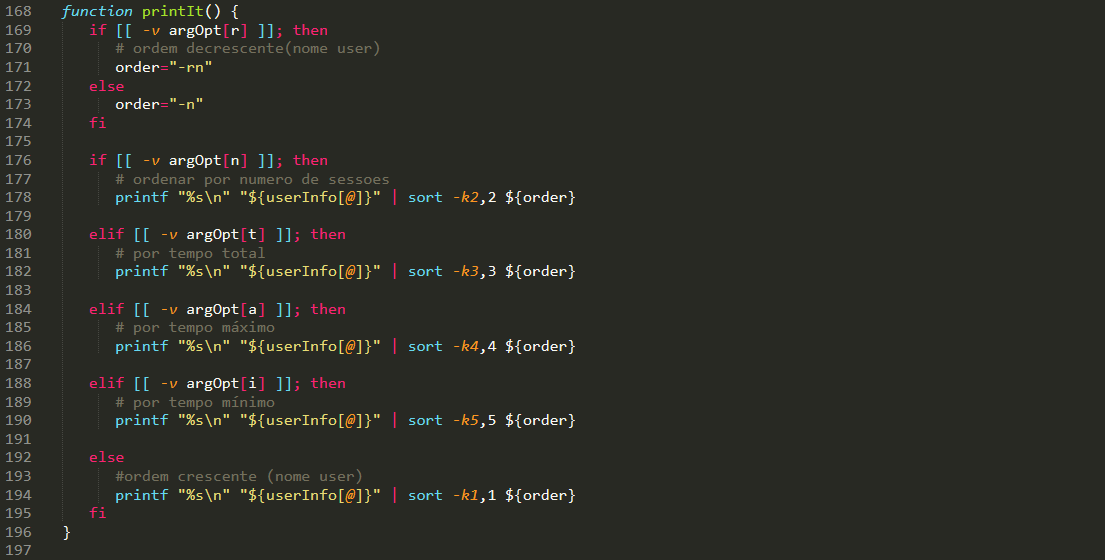
\includegraphics[width=\textwidth]{printit.png}
    \caption{Função \textbf{\textit{printIt()}} que procede à impressão dos dados tratados consoante a ordem desejada}
\end{figure}
\par O resultado ordenado dos dados filtrados é baseado na leitura e impressão, com a respetiva ordenação, dos dados dos \textit{Arrays Associativos} \textit{argOpt} e \textit{userInfo}.
\par No início da função, é verificada a existência da opção \textit{"-r"} no \textit{argOpt} através de uma expressão condicional com o operador \textit{-v}. Se isto acontecer, é criada uma variável chamada \textit{order} onde é guardado o valor \textit{"-rn"}, valor esse que permite aos \textit{printf}'s imprimirem as informações ordenadas de forma descrescente e numericamente. Em caso contrário, a variável \textit{order} vai apenas guardar \textit{"-n"} que ordena de forma crescente e numericamente.
\par As verificações seguintes averiguam qual opção de ordenação foi passada no \textit{argOpt}, de modo a imprimir no terminal os dados guardados em \textit{userInfo}, para cada utilizador, de acordo com o que foi introduzido como argumentos. Isto é feito com, além do \textit{printf}, o comando \textit{sort}, sendo que a opção \textit{"-k"} designa o local onde operar, daí ser seguido por dois números (por exemplo -k2,2), assegurando que a ordenação ocorre com a precedência da esquerda para a direita.



\clearpage
\section{Comparação das estatísticas dos utilizadores}
O script criado (\textit{comparestats.sh}) compara dois ficheiros que salvaguardam a saída do programa \textit{userstats.sh}. Após a sua execução, é possível observar a diferença entre os tempos de utilização e a diferença entre o número de sessões, considerando o primeiro ficheiro introduzido como o que representa os valores mais recentes. Os utilizadores que se encontram apenas num dos ficheiro também são apresentados.
\subsection{Estrutura}
\par Em semelhança ao script anterior, foram criados dois \textit{Arrays Associativos} e dois \textit{Arrays} para simplificar o tratamento dos dados.

\begin{figure}[!h]
    \centering
    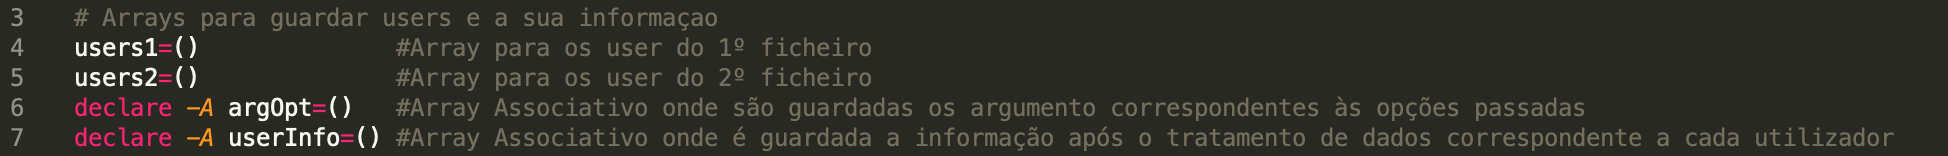
\includegraphics[width=\textwidth]{comparestats/estrutura_c.png}
    \caption{\textbf{\textit{Arrays}} mais relevantes na implementação deste script}
\end{figure}
\newline
 \begin{itemize}
   \item {\textbf{users1}}   - \textit{Array} onde são guardados os utilizadores, durante o tratamento de dados, correspondestes ao 1º ficheiro introduzido;
   \\
   \item {\textbf{users2}}   - \textit{Array} onde são guardados os utilizadores, durante o tratamento de dados, correspondestes ao 2º ficheiro introduzido;
   \\
   \item {\textbf{argOpt}}  - \textit{Array Associativo} onde são guardadas as opções e os respetivos argumentos durante o tratamentos de opções;
   \\
   \item {\textbf{userInfo}}- \textit{Array Associativo} onde são guardadas as informações tratadas durante o tratamento de dados.
 \end{itemize}
\clearpage

\subsection{Tratamento de Opções}
À semelhança do último script, as opções foram tratadas usando o comando shell \textit{getopts}, abordado nas aulas práticas.
\newline
\par O tratamento de opções é iniciado com a chamada da função \textbf{\textit{args()}}.
\begin{figure}[!h]
    \centering
    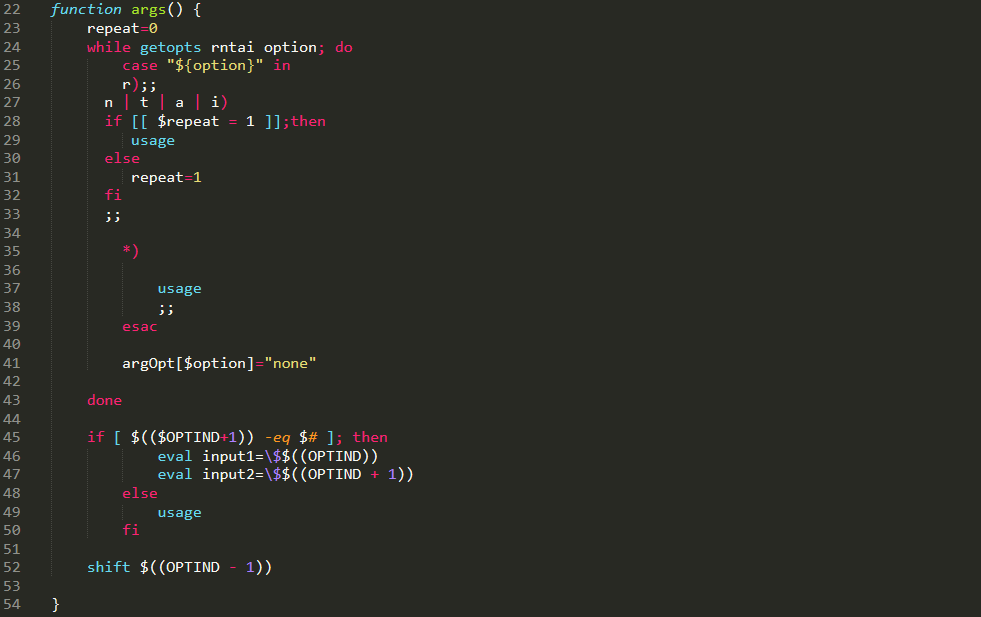
\includegraphics[width=\textwidth]{comparestats/getopts_c.png}
    \caption{Função \textbf{\textit{args()}} que procede ao tratamento de opções}
\end{figure}
\par O \textit{getopts} recebe parâmetros (\textit{rntai}) que correspondem às opções, neste caso sem argumentos, que o comando aceita. Estando este comando dentro de um \textit{while}, é repetido as vezes necessárias para percorrer todas as opções e argumentos introduzidos no programa. As opções são guardadas, em cada ciclo, na variável \textit{option} sendo executado o código associado a cada opção, consoante o \textit{case statement}.
\par Para as opções \textit{"-n"}, \textit{"-t"}, \textit{"-a"} e \textit{"-i"} que não podem ser repetidas, foi criada uma variável \textit{repeat} para averiguar se alguma destas variáveis já foi passada à função. Em caso afirmativo, é executada a função \textbf{\textit{usage()}}.
\par Sempre que é introduzida uma opção inválida ou de forma incorreta, o \textit{case statement} executa a função \textbf{\textit{usage()}}, que indica a forma de utilização do script.
\begin{figure}[!h]
    \centering
    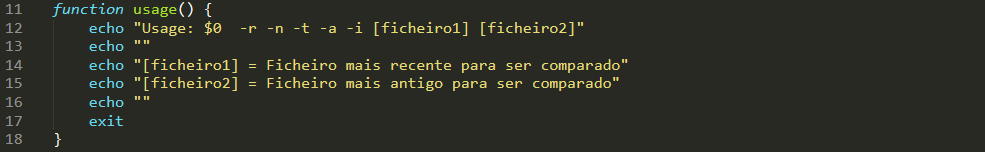
\includegraphics[width=\textwidth]{comparestats/usage_c.png}
    \caption{Função \textbf{\textit{usage()}} que refere as opções e argumentos esperados}
\end{figure}
\newline
\newline
\newline
\newline
\newline
\par Ainda dentro do \textit{while}, é adicionada a opção ao \textit{Array Associativo} \textit{argOpt}, se a função \textbf{\textit{usage()}} não tiver sido acionada antes.
\par Após o ciclo, é executada a verificação se \textit{\$((OPTIND+1))} é igual ao número de argumentos passado à função. Visto que a variável \textit{OPTIND} corresponde às opções e argumentos aceites no \textit{getopts}, incluindo o nome do ficheiro, e \textit{\$\#} corresponde ao número de argumentos passados ao script, com exceção do nome do ficheiro, é \textbf{incrementado um} ao \textit{OPTIND} de modo a comparar se o número de opções aceites no \textit{getopts}, com o nome dos dois ficheiros de texto, é igual ao número de argumentos, executando a função \textit{usage} em caso contrário. Assim, \textit{\$((OPTIND))} e \textit{\$((OPTIND+1))} correspondem, respetivamente, ao índice do argumento do primeiro e do segundo ficheiro.
\par Por fim, \textit{\$((OPTIND-1))} vai remover todas as opções que foram passadas pelo \textit{getopts}, nos seus parâmetros. Desta forma, \textit{\$1} vai referir o primeiro argumento passado ao script, que não é uma opção.


\clearpage

\subsection{Leitura e tratamento de dados}
\newline
\par Da mesma forma que a última implementação, o tratamento de dados é iniciado com a chamada da função \textbf{\textit{getUsers()}}.
\begin{figure}[!h]
    \centering
    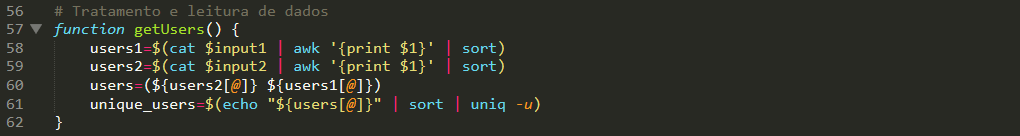
\includegraphics[width=\textwidth]{comparestats/getUsers_c.png}
    \caption{Função \textbf{\textit{getUsers()}} que procede ao armazenamento e seleção dos utilizadores}
\end{figure}
\par A função começa por fazer a impressão dos conteúdos de ambos os ficheiros através do comando \textit{cat}, sendo esta tratada pelo comando \textit{awk} que armazena nos \textit{Arrays} \textit{users1} e \textit{users2}, consoante o ficheiro, a primeira coluna da impressão. Visto que esta coluna corresponde aos utilizadores, estes \textit{Arrays} vão possuir os utilizadores contidos em cada um dos ficheiros, ordenados crescentemente, como dita o comando \textit{sort}.
\par Com o objetivo de criar um \textit{Array} dos utilizadores que não estão repetidos em nenhum dos ficheiro, entenda-se, únicos, foi criado o \textit{Array} temporário \textit{users} onde estão combinados os utilizadores de ambos os ficheiros. Posteriormente, para chegar ao resultado pretendido, foi criado um \textit{Array} \textit{unique\_users} que recebe a informação vinda da impressão do \textit{Array} \textit{users}, ordenada e apenas com os utilizadores únicos como é de esperar do comando \textit{uniq}, juntamente com a opção \textit{-u}, que não imprime as linhas repetidas. Tudo isto é auxiliado com a transformação de espaços por mudanças de linha \textit{tr '\hspace{0.2cm}'\hspace{0.2cm} '\textbackslash n'} para o comando \textit{uniq -u} tratar os dados, repondo a formatação no final.
\newline
\newline
\par Em seguida, a informação obtida passa para \textbf{\textit{getUsersInfo()}}.
\begin{figure}[!h]
    \centering
    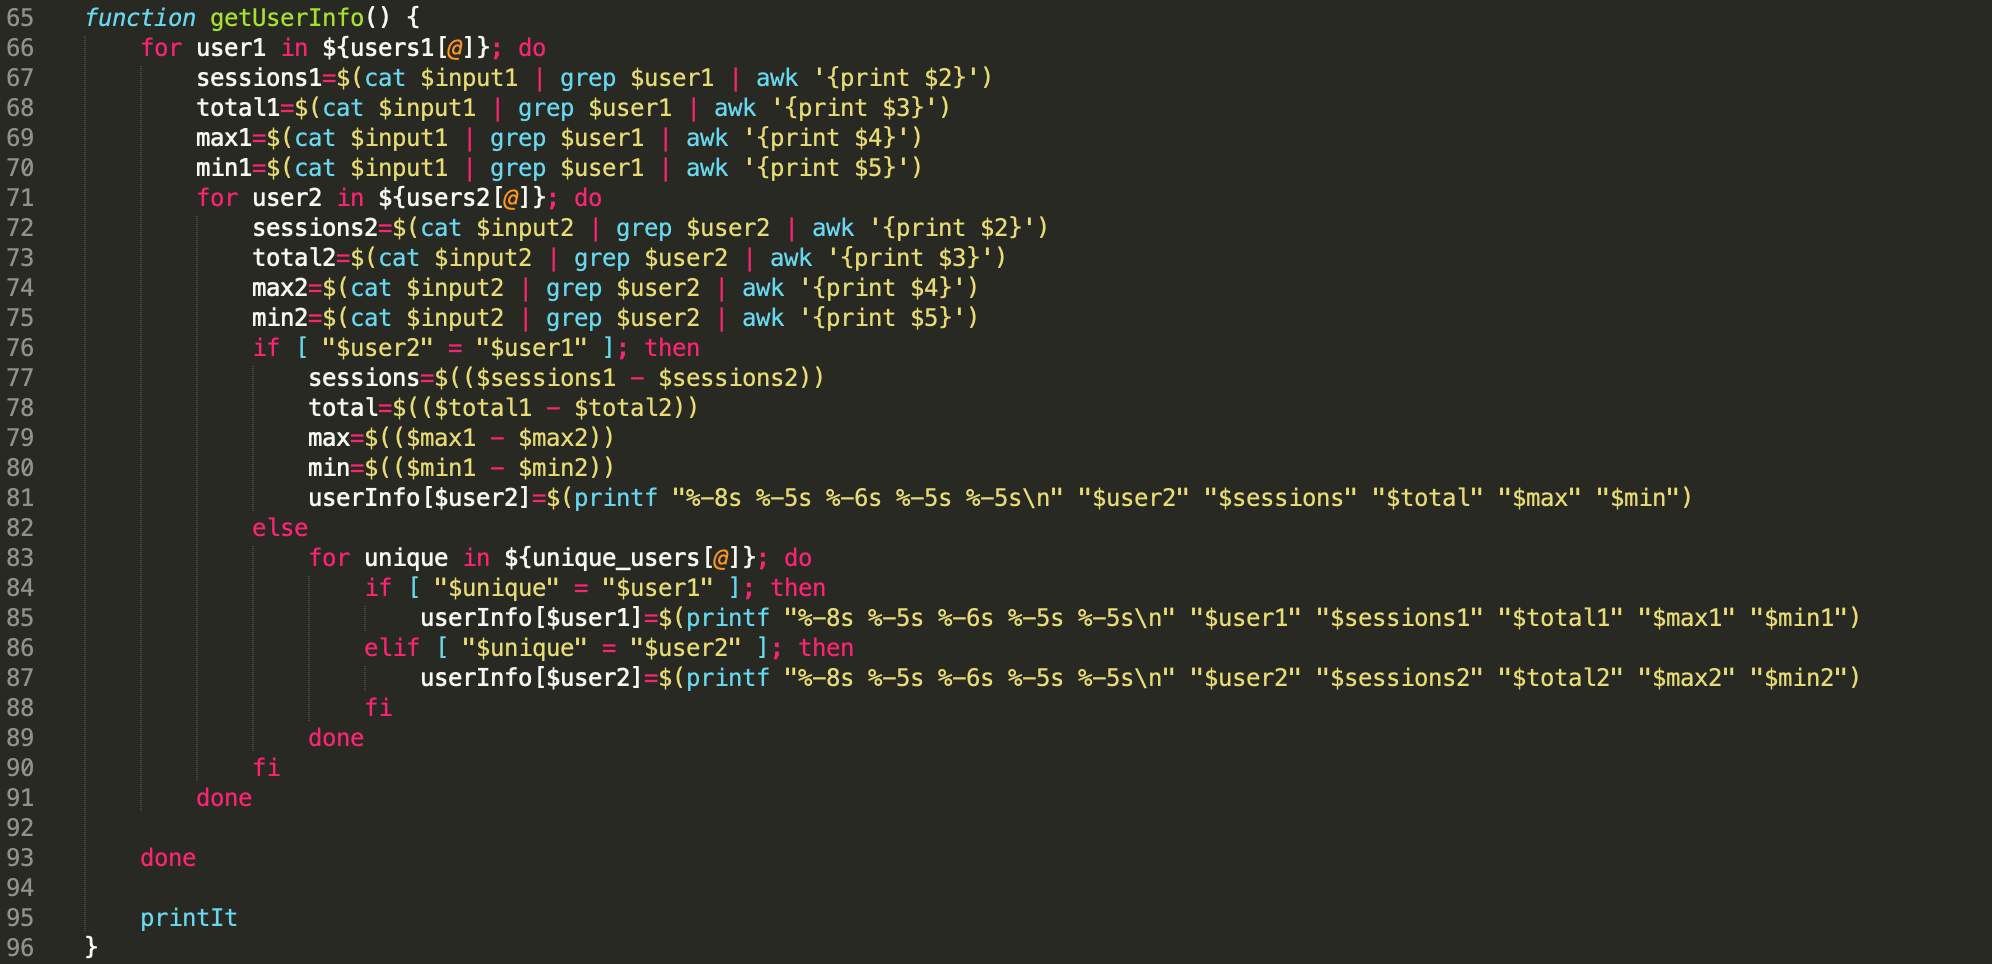
\includegraphics[width=\textwidth]{comparestats/getusersinfo_c.png}
    \caption{Função \textbf{\textit{getUsersInfo()}} que trata e calcula os valores pretendidos na impressão}
\end{figure}
\par O tratamento de dados do script consiste em percorrer todos os elementos de ambos os \textit{Arrays} criados na função anterior, comparar os valores e, tratar os mesmos. 
\par Isto é feito com dois ciclos \textit{for} que percorrem os utilizadores guardados anteriormente nos \textit{Arrays} \textit{users1} e \textit{users2}, guardando em \textit{Arrays} o número de sessões, o tempo total das sessões, o tempo máximo das sessões e o tempo mínimo das sessões correspondente aos utilizadores atuais do ciclo. Alcançou-se este propósito imprimindo novamente os ficheiros através do comando \textit{cat}, fazendo-se a seleção do utilizador atual do ciclo \textit{for} com o comando \textit{grep} e, por fim, a escolha da coluna correspondente aos dados em questão com o comando \textit{awk}. 
\Par A cada ciclo dos utilizadores do segundo ficheiro, é verificado se este utilizador é igual ao atual do primeiro ficheiro e, se isto se confirmar, são realizadas as subtrações dos valores do primeiro ficheiro com as do segundo, guardando essas informações no \textit{Array Associativo} \textit{userInfo}, à semelhança do último script. Em caso contrário, são percorridos os utilizadores únicos de modo a averiguar se este é pertencente ao primeiro ou ao segundo ficheiro, introduzindo os dados em \textit{userInfo}, consoante a verificação.

\clearpage

\subsection{Impressão ordenada dos dados filtrados}
\par A impressão ordenada dos dados filtrados é feita com a chamada da função \textbf{\textit{printIt()}} de igual forma ao script anterior.
\begin{figure}[!h]
    \centering
    
\includegraphics[width=\textwidth]{comparestats/printit_c.png}
    \caption{Função \textbf{\textit{printIt()}} que procede à impressão dos dados tratados consoante a ordem desejada}
\end{figure}
\newpage
Em ambas as implementações, estas funções são chamadas no fim do script, permitindo obter os resultados desejados.
\begin{figure}[!h]
    \centering
    
\includegraphics[width=\textwidth]{function_call.png}
    \caption{Chamada das várias funções em ambos os scripts}
\end{figure}
\newline
\par Com \textbf{\textit{args "\$@"}} é chamada a função \textbf{\textit{args()}}, juntamente com todos os argumentos passados no terminal, sendo que as outras duas funções são chamadas de seguida.
\clearpage
\section{Resultados}
\par Utilizando o computador da sala de aula, através de ligação remota, foram efetuados testes aos scripts desenvolvidos.
\par Ambos os scripts foram desenvolvidos a partir do comando \textit{last} ou de ficheiros derivados com os dados tratados.
\begin{figure}[!h]
    \centering
    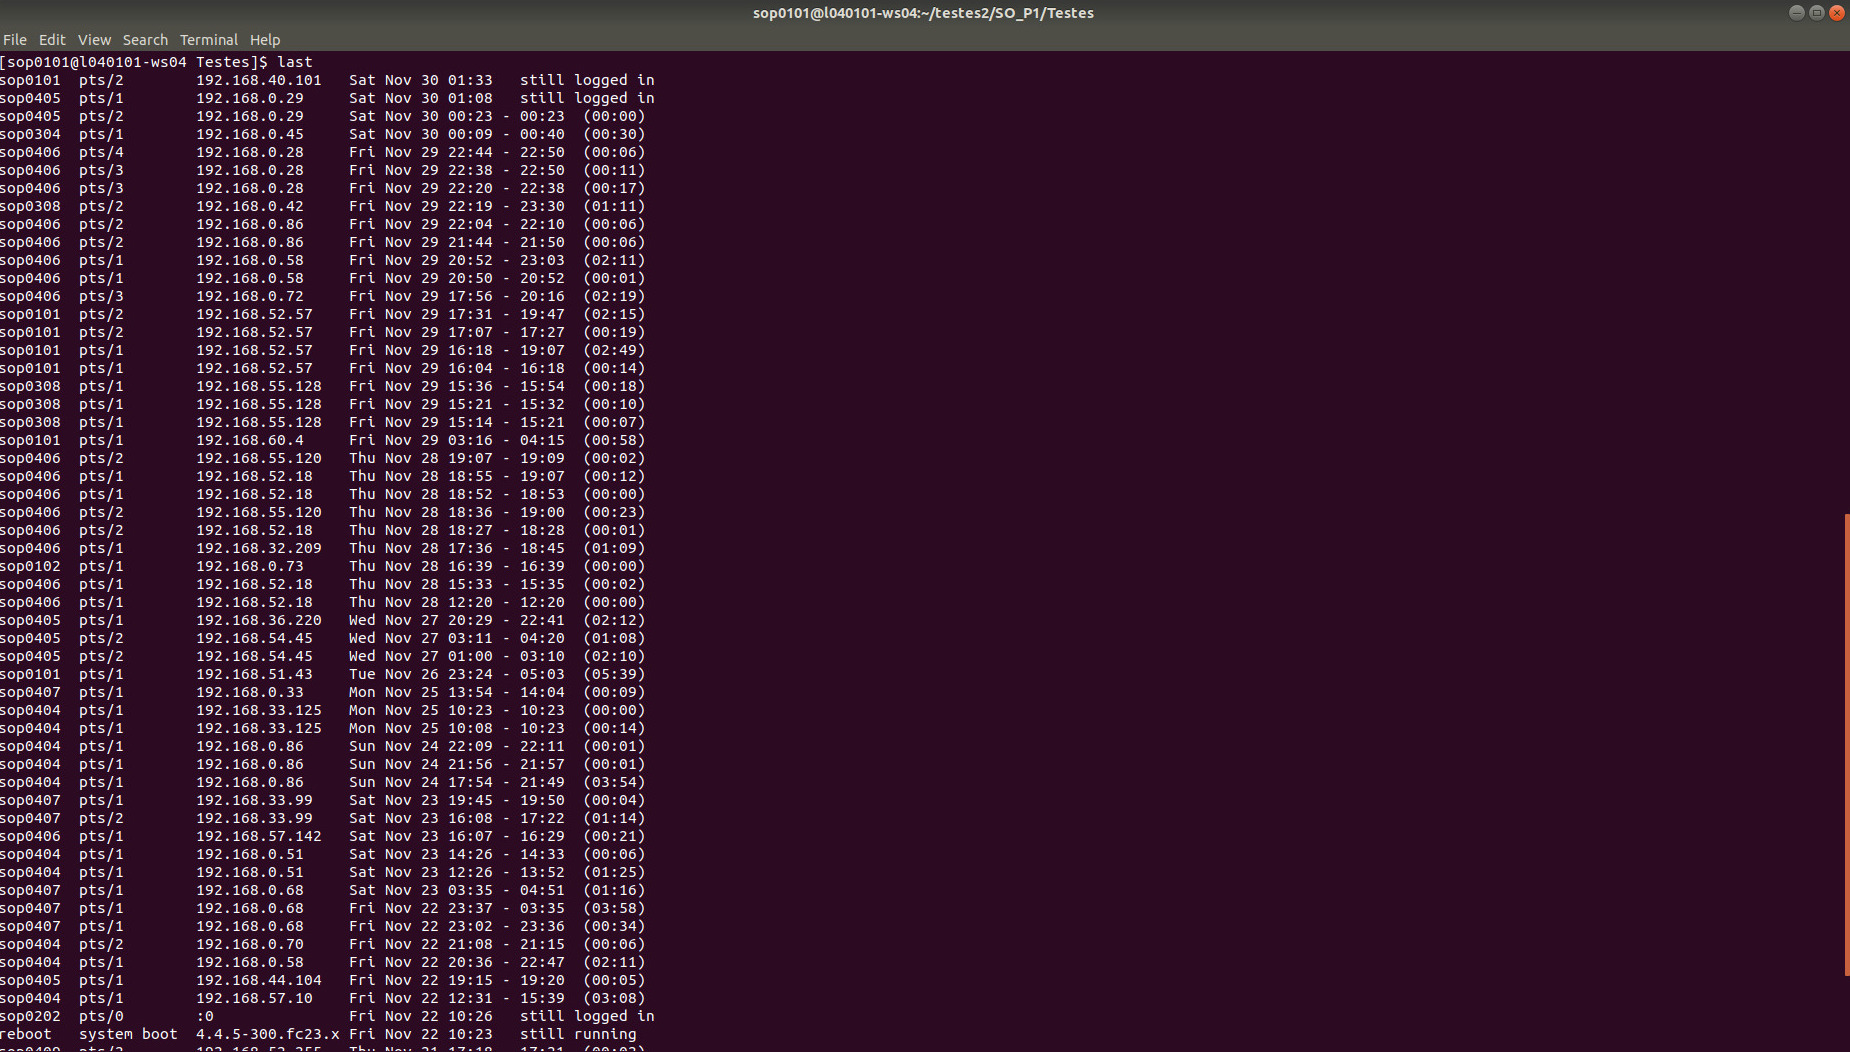
\includegraphics[width=\textwidth]{Resultados/last_1.jpeg}
    \centering
    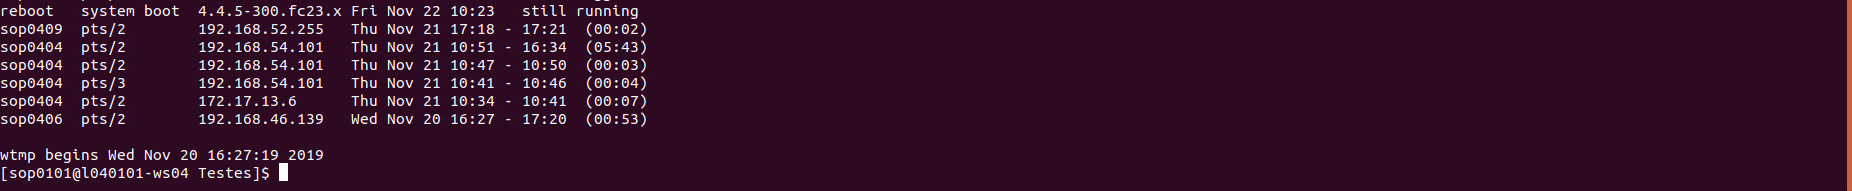
\includegraphics[width=\textwidth]{Resultados/last_2.jpeg}
    \caption{Execução do comando \textit{last} no computador da sala de aula, por volta das horas em que foram realizados os testes}
\end{figure}
\clearpage
\subsection{Estatísticas dos utilizadores}
\begin{figure}[!h]
    \centering
    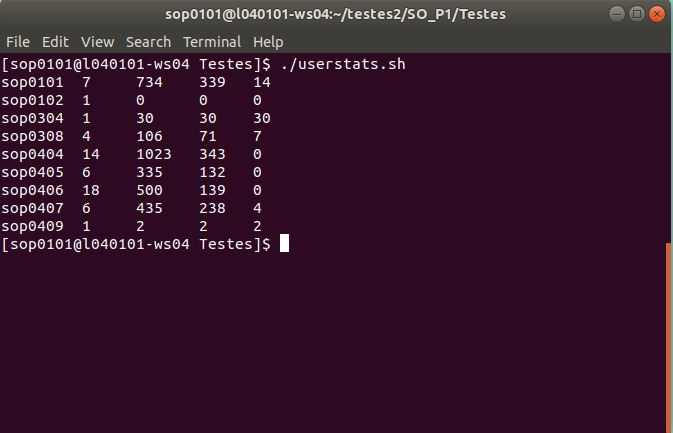
\includegraphics[width=350]{Resultados/normal.jpeg}
    \caption{Execução do script sem nenhum argumento}
\end{figure}

\begin{figure}[!h]
    \centering
    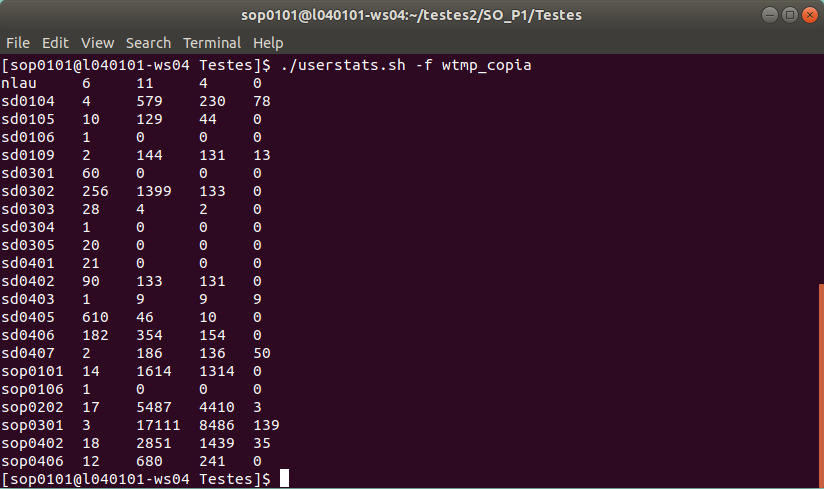
\includegraphics[width=350]{Resultados/user_f.jpeg}
    \caption{Execução do script com a opção \textit{-f} e a cópia do ficheiro"/var/log/wtmp", do computador da sala, (\textit{wtmp\_copia}) relativo a outra data }
\end{figure}

\begin{figure}[!h]
    \centering
    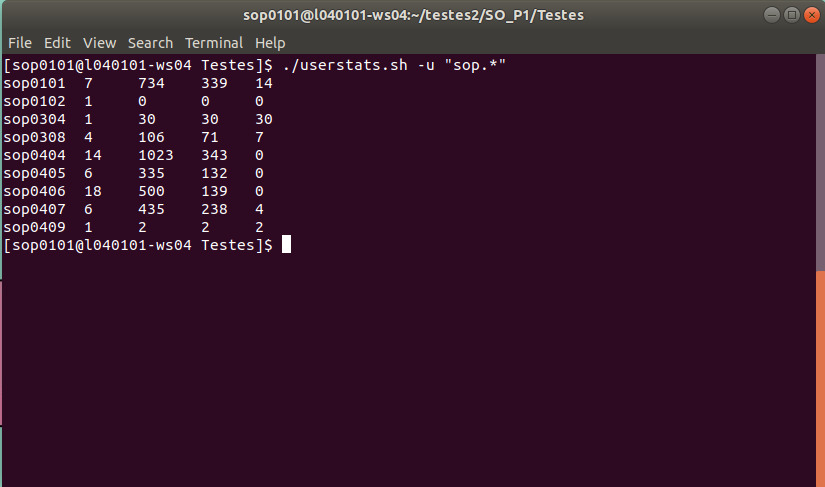
\includegraphics[width=350]{Resultados/user_u.jpeg}
    \caption{Execução do script com a opção \textit{-u} e o nome dos utilizadores para serem verificados através de uma expressão regular, neste caso \textit{"sop.*"}}
\end{figure}

\begin{figure}[!h]
    \centering
    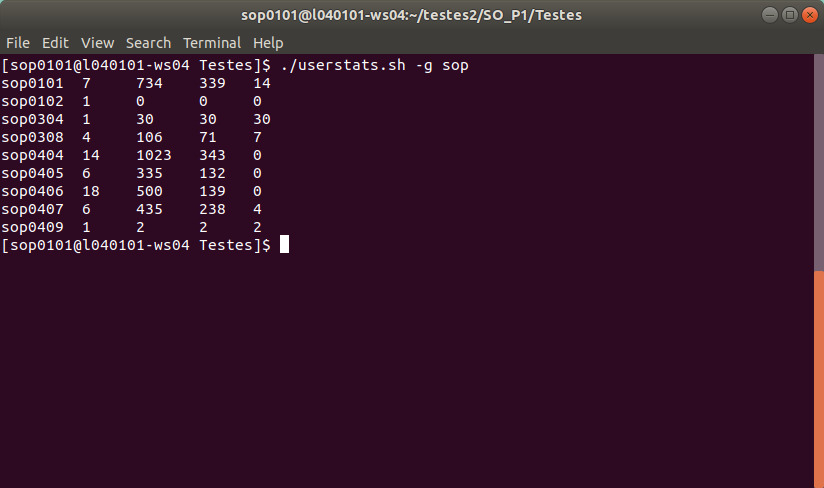
\includegraphics[width=350]{Resultados/user_g.jpeg}
    \caption{Execução do script com a opção \textit{-g} e o grupo a ser seleccionado, \textit{sop}}
\end{figure}

\begin{figure}[!h]
    \centering
    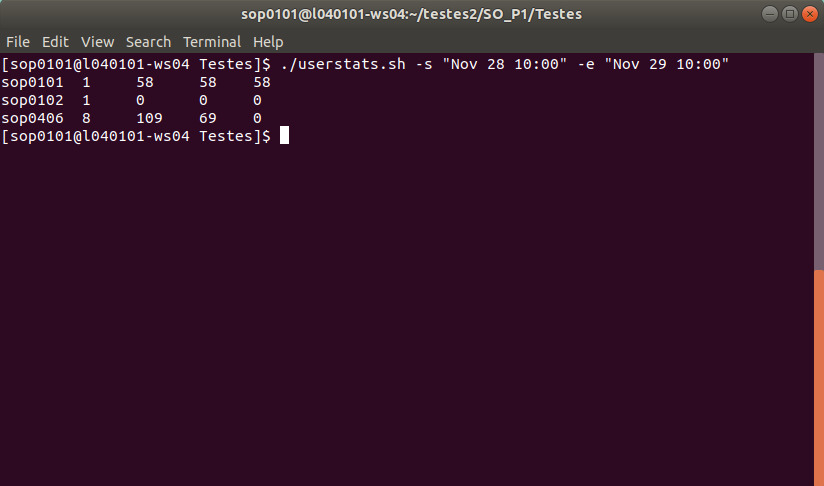
\includegraphics[width=350]{Resultados/user_s_e.jpeg}
    \caption{Execução do script com a opção \textit{-s} e \textit{-e} no intervalo de \textit{"Nov 28 10:00"}} a \textit{"Nov 29 10:00"}
\end{figure}

\begin{figure}[!h]
    \centering
    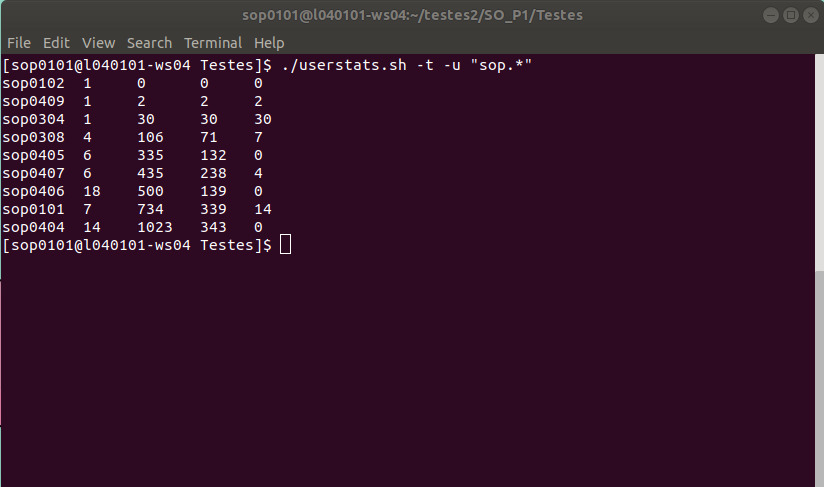
\includegraphics[width=350]{Resultados/user_t_u.jpeg}
    \caption{Execução do script com a opção \textit{-t} e \textit{-u} com o nome dos utilizadores para serem verificados através de uma expressão regular, neste caso \textit{"sop.*"}}
\end{figure}

\begin{figure}[!h]
    \centering
    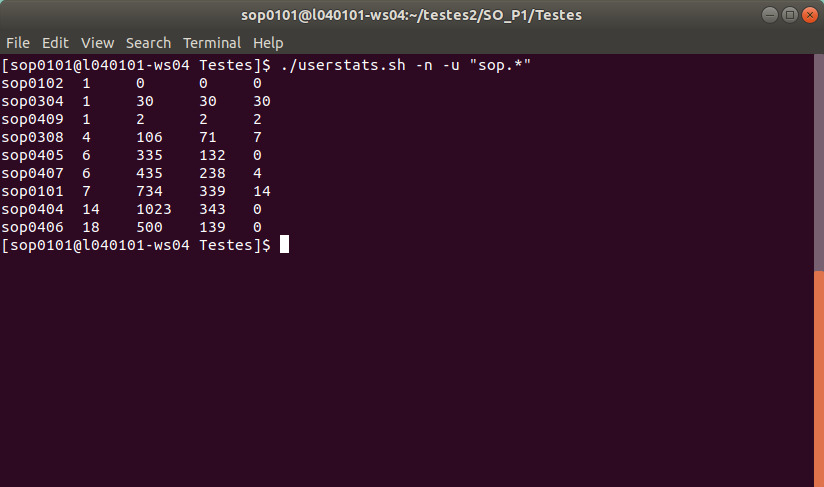
\includegraphics[width=350]{Resultados/user_n_u.jpeg}
    \caption{Execução do script com a opção \textit{-n} e \textit{-u} com o nome dos utilizadores para serem verificados através de uma expressão regular, neste caso \textit{"sop.*"}}
\end{figure}

\begin{figure}[!h]
    \centering
    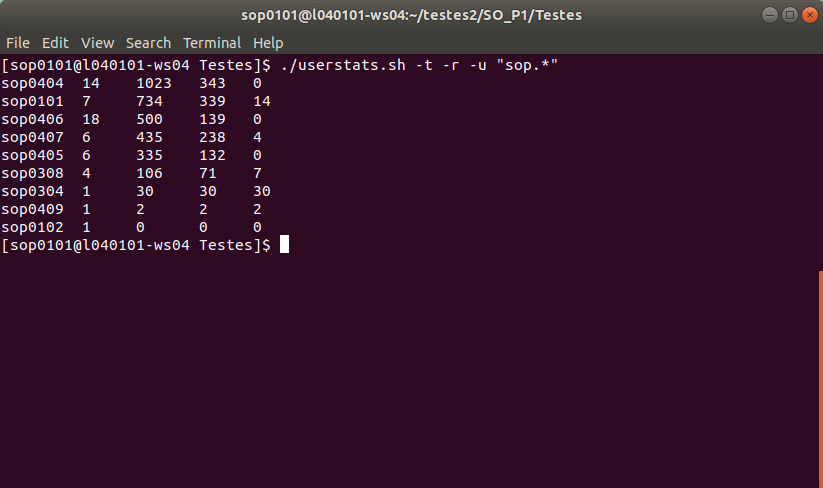
\includegraphics[width=350]{Resultados/user_t_r_u.jpeg}
    \caption{Execução do script com a opção \textit{-t}, \textit{-r} e \textit{-u} com o nome dos utilizadores para serem verificados através de uma expressão regular, neste caso \textit{"sop.*"}}
\end{figure}

\begin{figure}[!h]
    \centering
    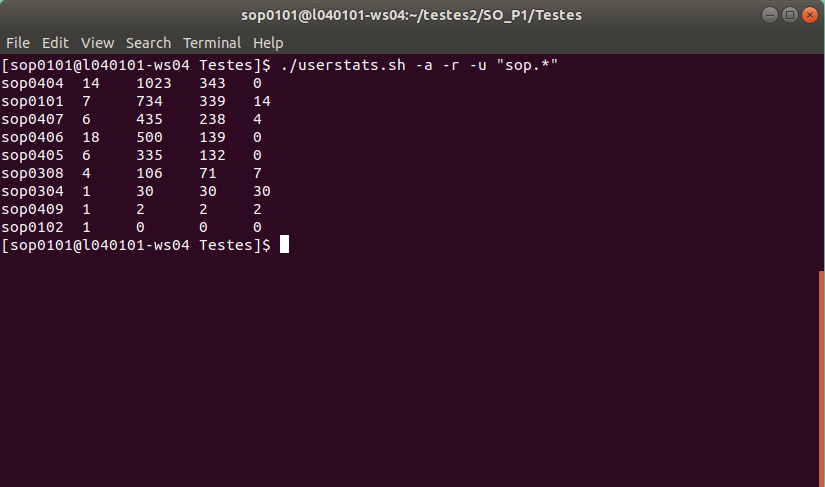
\includegraphics[width=350]{Resultados/user_a_r_u.jpeg}
    \caption{Execução do script com a opção \textit{-a}, \textit{-r} e \textit{-u} com o nome dos utilizadores para serem verificados através de uma expressão regular, neste caso \textit{"sop.*"}}
\end{figure}

\begin{figure}[!h]
    \centering
    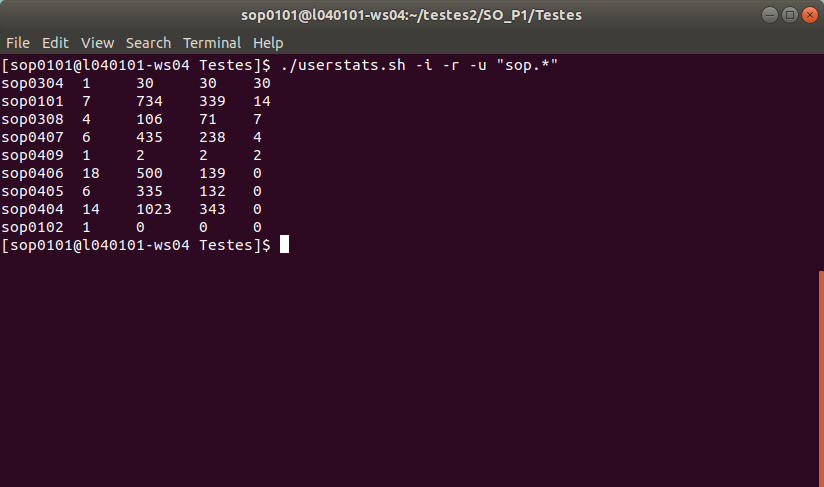
\includegraphics[width=350]{Resultados/user_i_r_u.jpeg}
    \caption{Execução do script com a opção \textit{-i}, \textit{-r} e \textit{-u} com o nome dos utilizadores para serem verificados através de uma expressão regular, neste caso \textit{"sop.*"}}
\end{figure}
\clearpage

No próximo teste foi introduzido um argumento juntamente com a opção \textit{-n}, que não recebe argumentos e, como é possível verificar, o tratamento de opções do script facilmente detetou o erro e chamou a função \textit{usage}.

\begin{figure}[!h]
    \centering
    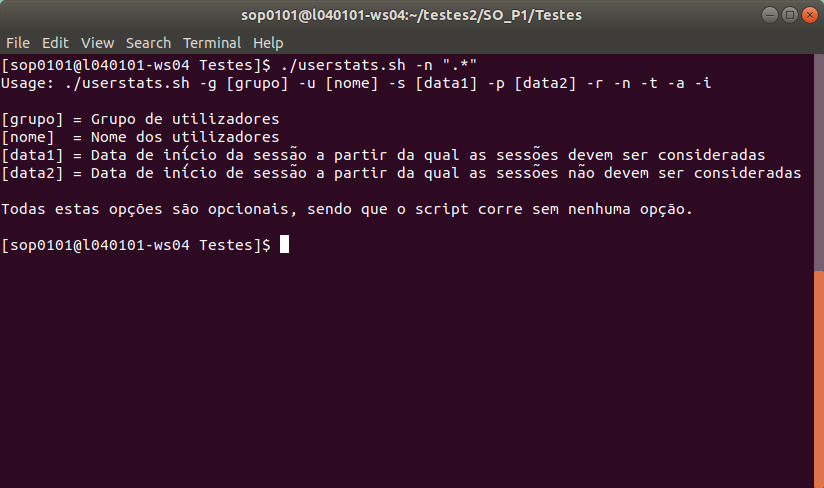
\includegraphics[width=350]{Resultados/usage.jpeg}
    \caption{Execução do script com a opção \textit{-n} e o argumento \textit{".*"}}
\end{figure}

Por fim, foi guardado o \textit{output} deste script, de modo a ser possível utilizá-lo no script seguinte.
\begin{figure}[!h]
    \centering
    
\includegraphics[width=350]{Resultados/save_cat.jpeg}
    \caption{Execução do script com a opção \textit{-n} e \textit{-u} com o nome dos utilizadores para serem verificados através de uma expressão regular, neste caso \textit{"sop.*"}, redirecionando o output para o ficheiro \textit{userstats\_20191130}}
\end{figure}
\clearpage
\subsection{Comparação das estatísticas dos utilizadores}
Os testes da comparação das estatísticas dos utilizadores foram realizados recorrendo aos outputs do script anterior. Foram utilizados ficheiro datados de \textit{23/11/2019} e \textit{30/11/2019}, sendo que foi considerado o primeiro aquele que possuía os valores mais recentes e portanto, as diferenças foram calculadas entre o primeiro e o segundo ficheiro.
\par A figura seguinte mostra o conteúdo de ambos os ficheiros, permitindo a sua análise antes da execução do script.
\begin{figure}[!h]
    \centering
    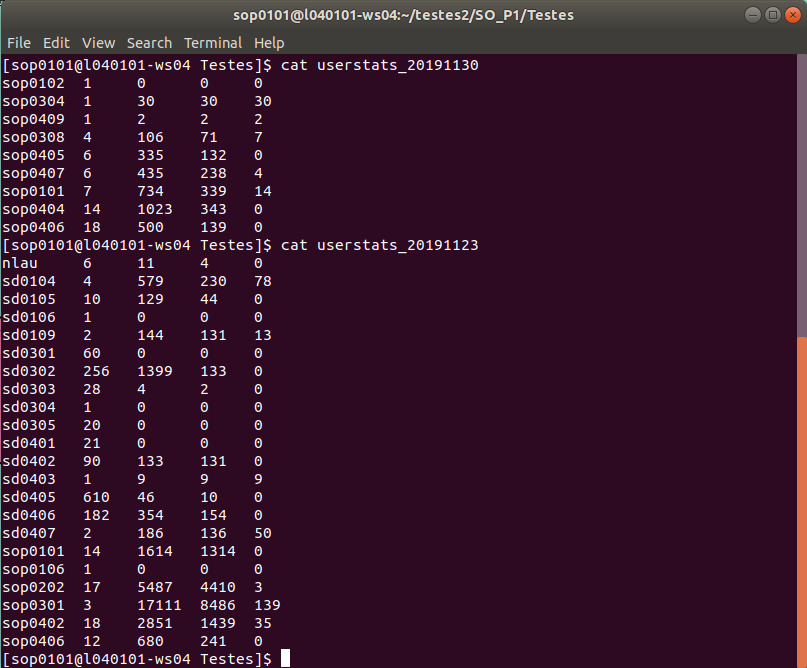
\includegraphics[width=300]{Resultados/cat_compare.jpeg}
    \caption{Impressão do conteúdo dos ficheiro \textit{userstats\_20191123} e \textit{userstats\_20191130}}
\end{figure}
\par É possível observar que apenas existem dois utilizadores iguais, em ambos os ficheiros. Desta forma, é possível prever o conteúdo que este script imprimirá, sendo que apenas efetuará os cálculos nestes utilizadores, mantendo os dados dos outros.

\begin{figure}[!h]
    \centering
    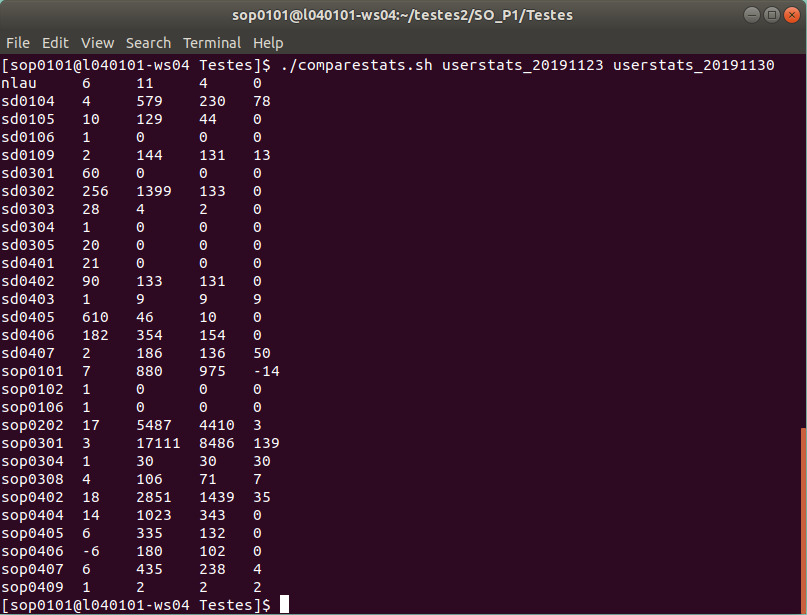
\includegraphics[width=300]{Resultados/normal_c.jpeg}
    \caption{Execução do script com os argumentos \textit{userstats\_20191123} e \textit{userstats\_20191130}}
\end{figure}

\begin{figure}[!h]
    \centering
    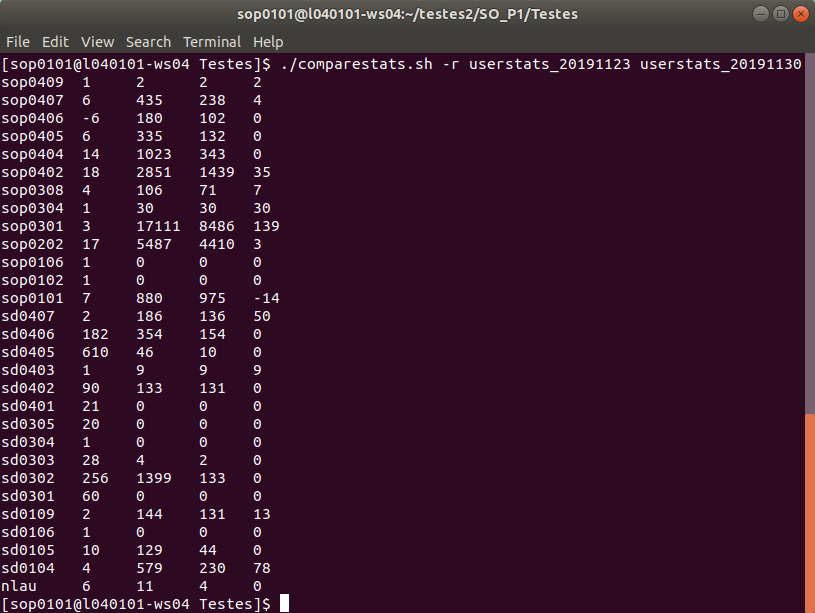
\includegraphics[width=300]{Resultados/compare_r.jpeg}
    \caption{Execução do script com a opção \textit{-r} os argumentos \textit{userstats\_20191123} e \textit{userstats\_20191130}}
\end{figure}
\begin{figure}[!h]
    \centering
    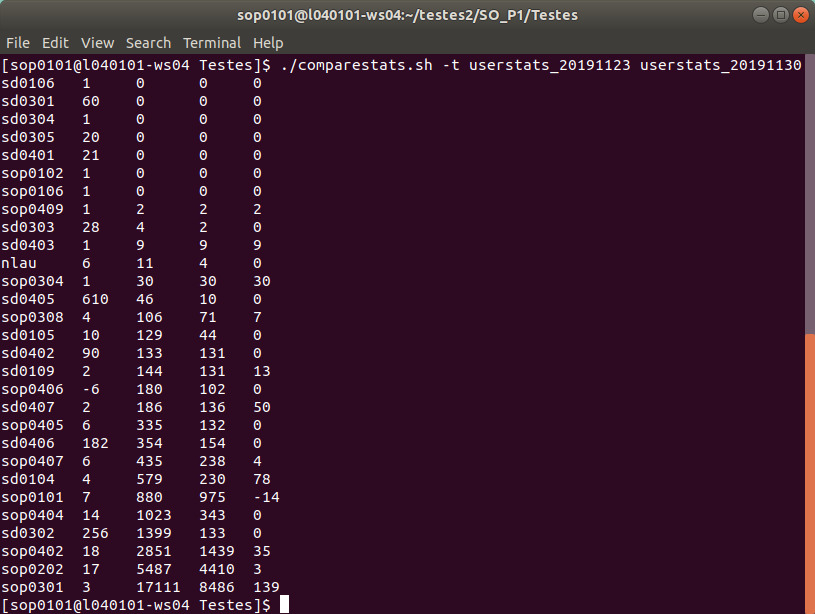
\includegraphics[width=300]{Resultados/compare_t.jpeg}
    \caption{Execução do script com a opção \textit{-t} os argumentos \textit{userstats\_20191123} e \textit{userstats\_20191130}}
\end{figure}

\clearpage

\section{Conclusão}
\par Em suma, os objetivos propostos pelo docente foram alcançados de acordo com as indicações dadas. A implementação foi pensada de forma a obter todos os resultados pretendidos, sendo que não houve grande incidência na otimização de código, uma vez que não era um dos requisitos. Ainda assim, tivemos em consideração, e tentámos, encontrar sempre soluções que não exigissem muito tempo de espera pelo output final. Considera-se, portanto, que a realização deste trabalho prático foi um sucesso.
\par Surgiram várias advertências pelo caminho, nomeadamente devido à especificidade da linguagem Bash, sendo que algumas das vezes se tornou complicado resolver, ou até mesmo encontrar, o problema em questão. Por vezes o problema era apenas falta de aspas em torno das variáveis, espaços nos sítios incorretos ou apenas um ciclo \textit{for} que não chegou a ser terminado, mas houve definitivamente vezes onde a procura de soluções chegou a demorar algumas horas. No entanto, tudo se encontra a funcionar mediante o trabalho proposto, sendo que o grupo acha que estas pequenas barreiras que foram aparecendo os obrigou a pesquisar e, consequentemente, a adquirir novos e mais vastos conhecimentos sobre diversos assuntos relacionados com esta linguagem.
\par Para além do referido, existiu outra advertência que condicionou a fase de testes. O grupo concluiu, ainda, que as configurações de ssh para as máquinas da sala de aula não se encontravam bem implementadas, impossibilitando a ligação aos computadores através de uma VPN da rede da Universidade. Deste modo, a realização dos testes teve de ser sempre realizada dentro da Universidade, trazendo alguns transtornos quando o trabalho se encontrava a ser desenvolvido fora da mesma. 
\par Quanto às estruturas de dados, concluiu-se que o uso de \textit{Arrays Associativos} em vez de \textit{Arrays} normais acabou por ser mais vantajoso, facilitando a manipulação dos dados.
\par Por fim, foi também concluído que existem vários utilizadores a recorrer ao computador em questão, maioritariamente ao final do dia e com sessões relativamente pequenas (menos de uma hora). Os grupos de utilizadores correspondentes a alunos, acabam por operar com muita frequência, devido à necessidade que estes têm para resolver questões escolares.


\clearpage

\section{Bibliografia}

\bibliographystyle{plain}

\bibliography{biblist}

\vspace{5mm} %5mm vertical space

[1] \url{https://pplware.sapo.pt/linux/personalize-a-prompt-de-comandos-da-Bash-no-linux/}

[2] \url{https://www.shellscript.sh/tips/getopts/}

[3] \url{https://www.gnu.org/software/Bash/manual/Bash.html}

[4] \url{https://aurelio.net/shell/canivete/}

[5] \url{https://stackoverflow.com}

\end{document}

